\documentclass{article}

\setlength{\parindent}{0pt}
\usepackage[round]{natbib}
\usepackage{listings}
\usepackage{array}
\newcolumntype{P}[1]{>{\centering\arraybackslash}p{#1}}

\usepackage{graphicx}
\graphicspath{ {./images/} }

\usepackage[font={small}, skip=3pt]{caption}

\title{Simulation of Tree Growth}
\date{2020-12-01}
\author{Eric Ekström}
	
\begin{document}
	
	\pagenumbering{gobble}
	\maketitle
	\newpage
  	\tableofcontents
  	\newpage
  	\pagenumbering{arabic}

  	\section{Introduction}
  	
  	Creating realistic tree assets for computer graphics by hand is a time consuming task. Various methods exist for automating the task. Methods for procedural generation of trees can be divided into two groups. Descriptive methods aim to create trees without considering how a tree might evolve to look a certain way. Mechanistic methods model the growth of a tree over time, considering factors that might affect how a tree evolves. \\
  	
  	This project aims to combine previous work on mechanistic tree generation and implement a method for generation of procedural trees in c{\small++} using opengl. This method is largely based on the work by \cite{palubicki2009self} with influences from \cite{mvech1996visual} and \cite{yi2018tree}. \\
  	
  	Along with the generation of trees, a number of interesting opengl lighting techniques were implemented, with the most prominent being volumetric light scattering.
  		 
  	\section{Background}
  		
  		This section covers the relevant background information related to the generation of trees and lighting phenomenon. It also covers terminology used throughout the report. 
  		
  		\subsection{Tree Structure and Terminology}
  			This section covers the terminology used when describing trees. The choice of language is based on the description of trees by \citep{barthelemy2007plant}. \\
  			
  			A tree consists of a number of nodes. Each node supports nodes further out in the tree, creating a graph structure of interconnected nodes.
  			
  			\begin{itemize}
  				\item A \textit{node} is the main component of the tree. It supports at least a bud, another node or a leaf. A node combined with an internode is called a \textit{metamer}. \citep{barthelemy2007plant}
  				\item An \textit{internode} is the section of stem between two nodes.
  				\item The \textit{lateral branch} is a supported node that is connected at an angle  to the supporting node.
  				\item The \textit{main branch} is a supported node that has the same angle as the supporting node.
  				\item \textit{Buds} are potential points for expansion of new nodes. A lateral bud is located at the node that already has a main branch. An apical bud is located at a node that has no branches to support.
  				
  			\end{itemize}
  			
  			For this project, a tree grows by shooting a number of new metamers from a bud for each iteration of growth. This is called rhythmic growth and is the more commonly observed method of growth in nature. \citep{barthelemy2007plant} The fate of a bud and the number of new metamers depends on a number of factors. For this project, only a simulated light resource was considered.\\
  			
  			A node is given an order based on the number of node below it. A node without a supporting node has order one.
  		\subsection{Volumetric Light Scattering}
  			Volumetric light scattering (also called "godrays" or "crepuscular rays") is a light phenomenon that occurs when the mixture of gas and molecules in the air is just right. This causes light to be rayleigh-scattered and creates visual sun beams through the air. (Figure \ref{fig:godrayexample})
  			
  			\begin{figure}[h!]
  				\centering
  				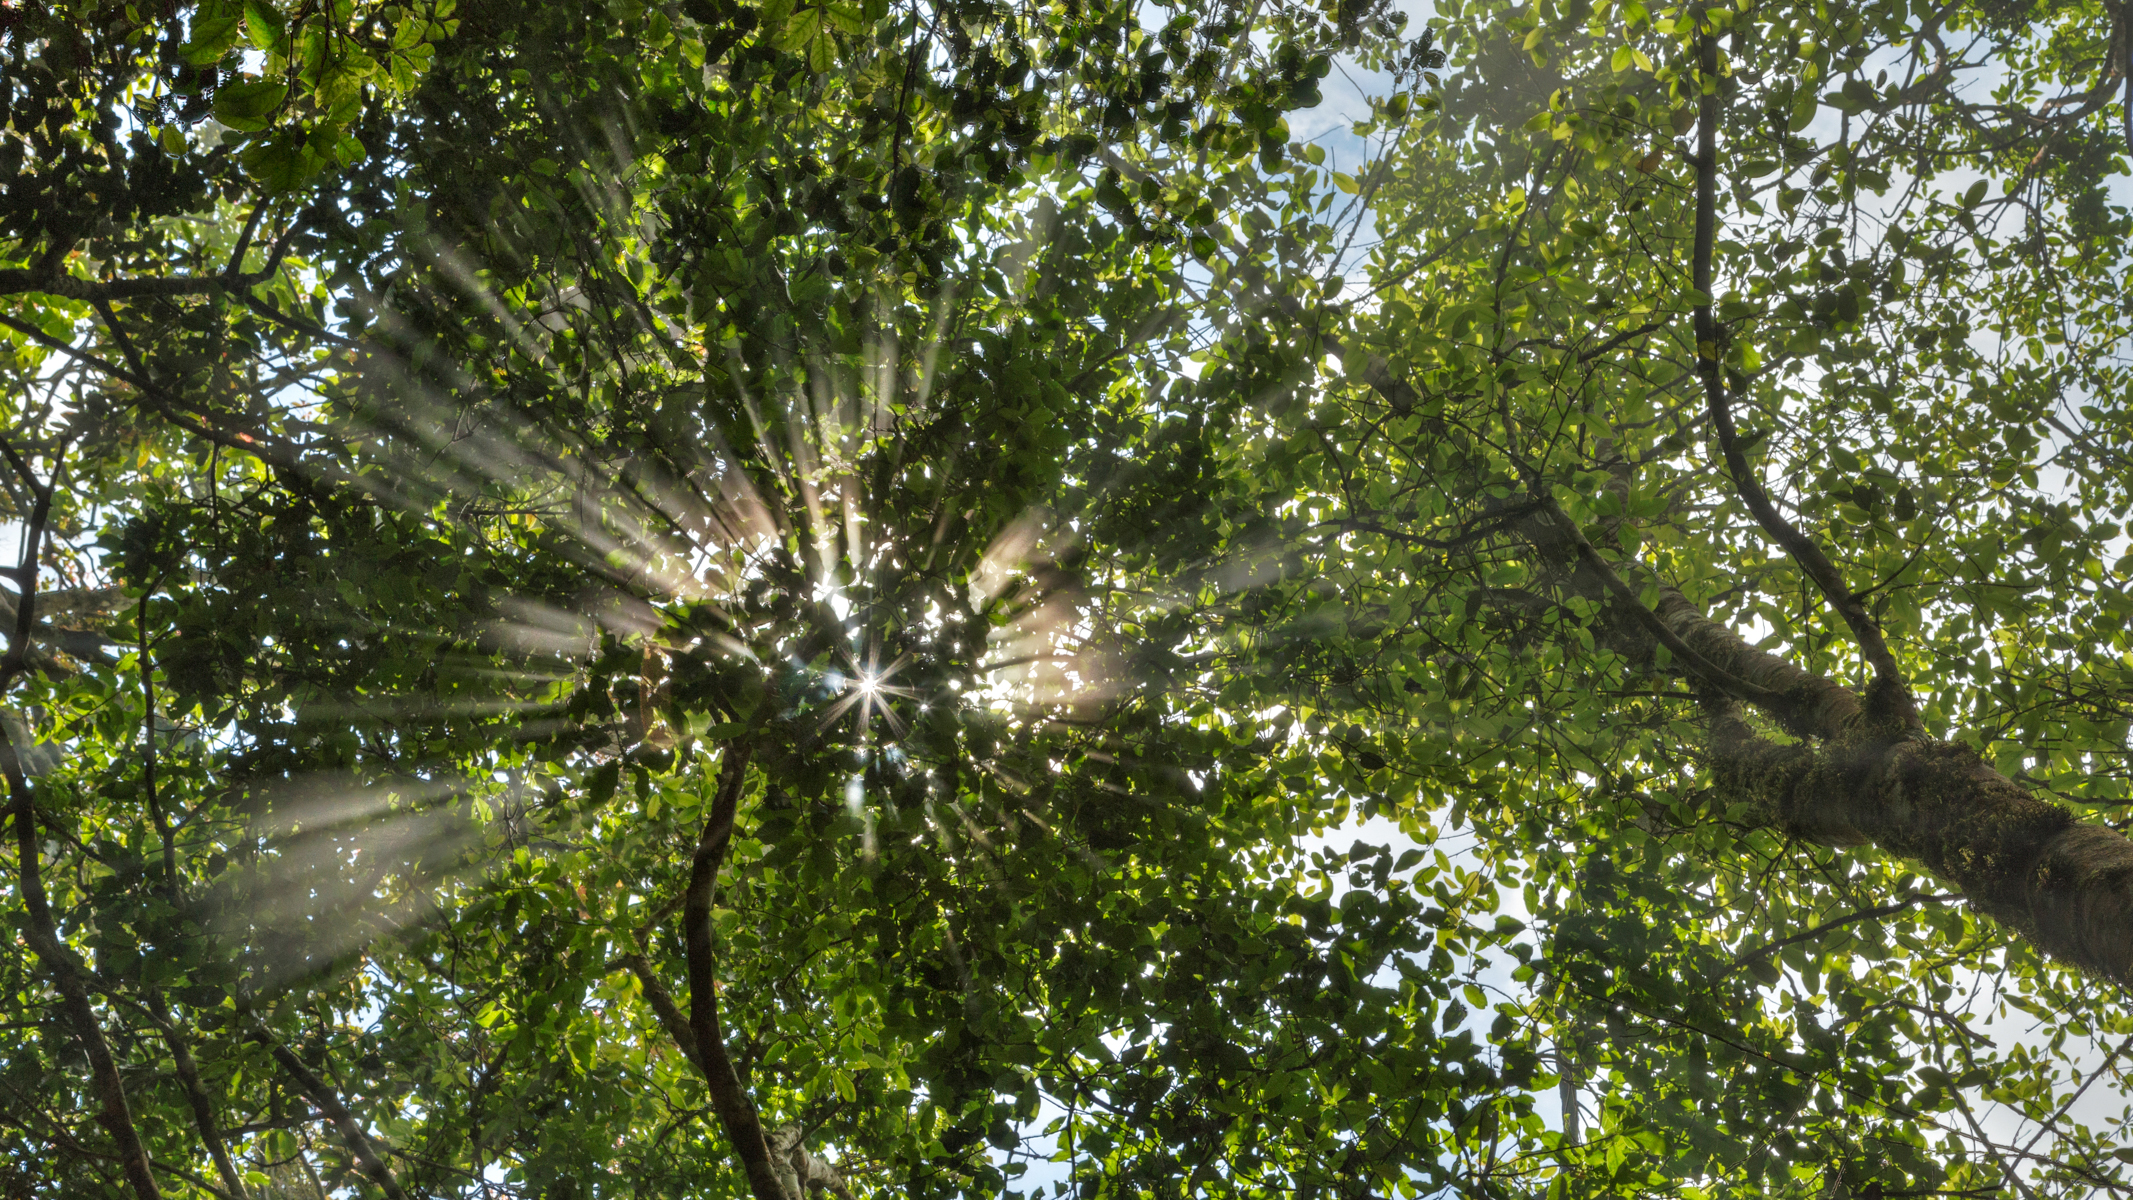
\includegraphics[scale=0.7]{godrays_example}
  				\caption{An example of volumetric light scattering. (Sunshine Kodai Kanal, Manoj K Racherla, 2013)}
  				\label{fig:godrayexample}
  			\end{figure}
  			
  		
  			
  	\section{Method}
  		\subsection{Tree Generation}
  			
  			The tree generation algorithm is an iterative process where each iteration grows the tree an amount. Each step in the algorithm outline below is implemented as a recursion of the node structure which changes each node or collect information.
  			
  			\subsubsection*{Algorithm outline}
  			
  			The tree generation algorithm used the same basic steps as described by Wojciech Palubicki. \citep{palubicki2009self}
  			
  			\begin{enumerate}
  				\item Calculate the amount of light resources available in the tree.
  				\item Redistribute light resources and create new nodes.
  				\item Update the branch radii for each node.
  				\item Calculate which nodes are a liability, and shed those.
  			\end{enumerate}
  		
  			\subsubsection*{Calculation of light resources}
  			
  				Light resources are collected from each node and saved in the base of the tree. Each node contribute with resources if it has either a lateral or apical bud. The size of the contribution is calculated according to Equation \ref{eq:lightres} as proposed by \cite{yi2018tree}. \textit{T} and \textit{$T_0$} is the current time and the creation time of the node respectively, \textit{l} is the light that hits the current node based on conditions around it and $\sigma$ is a controllable parameter.
  				
  				\begin{equation}
  					\label{eq:lightres}
  					Q = l^{{(T-T_0)}^\sigma}
  				\end{equation}
  				
  				Each node also has a cost associated with it. This is the amount of resources it takes to keep the node alive as described by \cite{mvech1996visual}. The equation for calculating this factor is shown in Equation \ref{eq:nodecost}. \textit{BM} and BE are control parameters. This factor is subtracted from the light resources in each node before the result is propagated to the supporting node. 
  				
  				\begin{equation}
  					\label{eq:nodecost}
  					BM * {\frac{radius}{default\_radius}}^{BE}
  				\end{equation}
  				
  			\subsubsection*{Shadow propogation for node light calculation}
  				
  				The variable \textit{l} in equation \ref{eq:lightres} is the amount if light that reach a node and is calculated by considering the nodes already around it. This is done by dividing the space into \textit{voxels} of fixed size. Each voxel saves a float value describing how shadowed the point is. When a new node is added to the tree, it also updated the voxels around it. Specifically, a pyramid of voxels (with the voxel containing the new node at the top) are updated according to Equation \ref{eq:shadowprop}. \textit{a} and \textit{b} are controllable parameters and \textit{q} is the number of voxels down from the top of the pyramid. \citep{palubicki2009self}
  				
  				\begin{equation}
  					\label{eq:shadowprop}
  					s = s_{prev} + a*b^{-q}
  				\end{equation}
  			
  			\subsubsection*{Redistribution of light resources}
  				An adapted version of the Borchert-Honda (BH) model \citep{borchert1984control} was used to redistribute resources to each node. The BH model was originally developed to control distribution of growth-inducing resources. \cite{palubicki2009self} adapted the BH model by using the collected light resources to guide the redistribution of resources. Equation \ref{eq:vm} and \ref{eq:vl} show how the light resources are distributed between the main branch and the lateral branch  based on the amount of resources collected by each node. $Q_m$ and $Q_l$ is the amount of light resources collected by each of the branches and $\lambda$ is a parameter that can be set by the user.
  			
	  			\begin{equation}
	  				\label{eq:vm}
	  				v_m = v\frac{\lambda Q_m}{\lambda Q_m + (1 - \lambda)Q_l}
	  			\end{equation}
	  			
	  			\begin{equation}
	  				\label{eq:vl}
	  				v_l = v\frac{(1 - \lambda) Q_l}{\lambda Q_m + (1 - \lambda)Q_l}
	  			\end{equation}
	  			
	  			The number of new metamers created from a bud is the integer part of the amount of resources that reach the bud. Three factors are considered when deciding the direction of the new branch; direction of the parent node, the optimal growth direction, and a tropism factor. The tropism factor, $\tau$, simulate how much the branches bend down due to gravity. The optimal growth direction  is found as the neighboring shadow voxel with the lowest value. These three factors are combined to the final growth direction according to Equation \ref{eq:growthdir}. \citep{palubicki2009self}
	  			
	  			\begin{equation}
	  				\label{eq:growthdir}
	  				growth\_dir = 0.8 * parent\_dir + 0.2 * optimal\_dir + \tau
	  			\end{equation}
	  			
	  		\subsubsection*{Update branch radii}
	  			
	  			The radius of each branch is updated to support the weight of the branches above it according to Equation \ref{eq:radius}, where $r_m$ and $r_l$ are the new radius of the supported branches. If no supported branch is present, the default branch radius is used. \citep{mvech1996visual}
	  			
	  			\begin{equation}
	  				\label{eq:radius}
	  				r = \sqrt{r_m^2 + r_l^2}
	  			\end{equation}
	  			
	  		\subsubsection*{Calculate shedding branches}
	  			
	  			A branch is shedded if the light resource flowing through it is negative and the number of supported buds are less than a threshold.
	  			\citep{mvech1996visual}
	  		
	  		
	  		\subsubsection*{Tree Parameters}
	  		
	  		Table \ref{table:param} shows the parameters that are available in the tree generation and how they affect the look of the tree. The most important parameters for controling the apperance of a tree is the branch bias factor, $\lambda$ and the tropism factor, $\tau$.
	  		
	  		\begin{table} [!h]
	  			\begin{center}
	  				\caption{Table of used tree parameters.}
	  				\begin{tabular}{ | c | m{6.5cm} | c | } 
	  					\hline
	  					\textbf{Name} & \textbf{Effect} & \textbf{Reasonable range} \\
	  					\hline
	  					lambda, $\lambda$ & Branch bias. Larger value gives priority to main branches. & 0.4 - 0.5 \\ 
	  					\hline
	  					sigma, $\sigma$ & Light conversion rate. Larger values increase the amount of light an older node can pick up. & 0 - 1\\ 
	  					\hline
	  					tropism, $\tau$ & Larger value bend branches more towards the ground. & 0.01 - 0.5 \\ 
	  					\hline
	  					BM & Branch maintenance coefficient & 0.01 - 0.5 \\ 
	  					\hline
	  					BE & Branch maintenance exponent &  $>$1\\ 
	  					\hline
	  					$N_{min}$ & Threshold for branch shedding. & 20 - 50 \\ 
	  					\hline
	  				\end{tabular}
	  				
	  				\label{table:param}
	  			\end{center}
	  		\end{table}
  		
  		
  			\subsubsection*{Tree rendering and OpenGL}
  			
  				The tree stem is rendered as cylinders with a different radius in each end. The bottom radius is the radius of the current node, while the top radius is the max radius of the two supported nodes. Each leaf uses the same mode which is then rotated to fit the position of the branch. All leafs in a tree are rendered as a part of one instanced draw call. This optimizes the rendering quite substantially. 
  			
  		\subsection{Volumetric Light Scattering}
  		
  			Volumetric light scattering was done as a post-process shader using the method described by Kenny Mitchell \citep{mitchell}. \\
  			
  			The post-process shader combines the normal render pass with a render pass where the sun is rendered as a single color, and all other objects are then rendered black. This gives an image with color only where the sun is visible from the cameras perspective. \\
  			
  			The post-process shader sums samples of the volumetric light scattering pass from the current fragment point to the position of the sun. The samples are exponentially weighted where the samples close to the sun are weighted higher. The equation used for weighting samples is shows in Equation \ref{eq:godray}. 
  			
  			\begin{equation}
  				\label{eq:godray}
  				L = exposure * \sum_{i = 0}^{n} decay^i * weight * \frac{sample}{n}
  			\end{equation}
  			
  			\textit{n} is the number of samples between the fragment position and the sun position, \textit{decay} is the exponentially decaying factor that dissipated the contribution from each sample. The \textit{exposure} and \textit{weight} factors are simply scale factors that increase or decrease the final light. \\
  			
  			The final factor \textit{L} for each pixel is then added to the final color of the normal pass for that pixel. The shader code used for volumetric light scattering can be found in appendix \ref{appendix:godray}.
  		
  		\subsection{Shadow Mapping}
  			Shadow mapping is a popular technique for generating good shadows in a scene. It works in two steps; first render the scene from the perspective of the light source, then render the scene as normal using the first render to calculate which fragments are in shadow. \citep{ragnemalm2015so} \\
  			
  			The purpose of the first render pass is to generate a map of depth values for each point that the camera can see. These depth values are then used in the second pass to calculate shadows. If the distance to the camera from the current fragment is greater then the depth value saved in the depth map, there is another fragment somewhere in between the fragment and the sun and the fragment is therefor in shadow. \citep{ragnemalm2015so}
  			
  			\subsubsection*{Implementation}
  				
  				A framebuffer with only a depth attachment was used to generate the depth map. Since the only part of interest is the depth values, the used fragment shader can be empty and just write the depth values to the z-buffer. The vertex shader is the same as would be used in a normal scene. \\
  				
  				The implementation for this project only create shadows from directional light sources. Because of this, a orthographic projection matrix was used. This gives a more realistic result by pretending that all light hits the scene as parallel lines. The position of the light source still have to de specified since it is needed to calculate the distance from a fragment. \\
  				
  				This method will generate a number of different artifacts that have to be addressed. The first and most obvious is "shadow acne". This is caused by the fact that the resolution of the shadow map is limited and there is more than one fragment on a surface that sample from the same point in the shadow map. Even though all the fragment on a surface should be lit, only the fragments that happen to have its distance saved in the shadow map are actually lit. This can be solved by adding a small offset when comparing the distance with the depth map. \\
  				
  				The next problem that has to be handled is the fragments that are outside the depth map. here we simply set the texture as "clamp to edge" and set the border of the depth texture to 1. The same problem arise when a fragment is beyond the outer limit of the projection matrix. The solution is to set the shadow to 0 if the distance is greater than the furthest allowed distance.
  				
  				For a full implementation of the shader code used for shadow mapping, see appendix \ref{appendix:shadow}.
  				
  	\section{Result}
  		
  		This sections present selected results of the tree generation and lighting effects. A list of all parameters used for various trees can be found in Table \ref{table:usedparam}. \\
  		
  		The growth process of a tree can be seen in Figure \ref{fig:treegrowth}. Notice the branch to the lower left. It clearly shows the growth of an individual branch over time. \\
  		
  		\begin{figure}[t]
  			\centering
  			
\includegraphics[height=6cm]{treegrowth1}
  			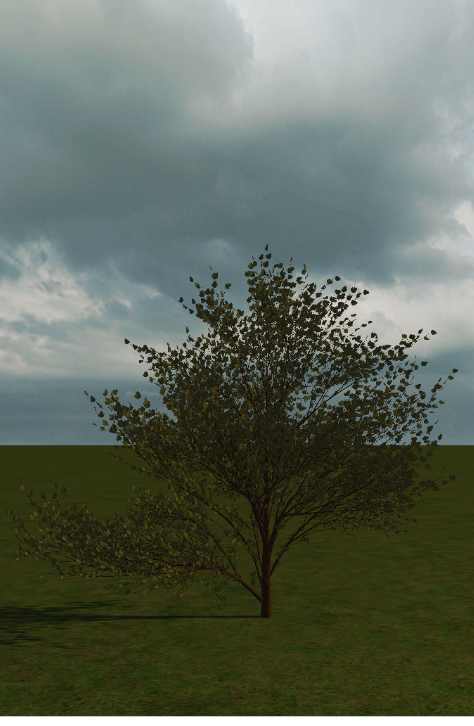
\includegraphics[height=6cm]{treegrowth2}
  			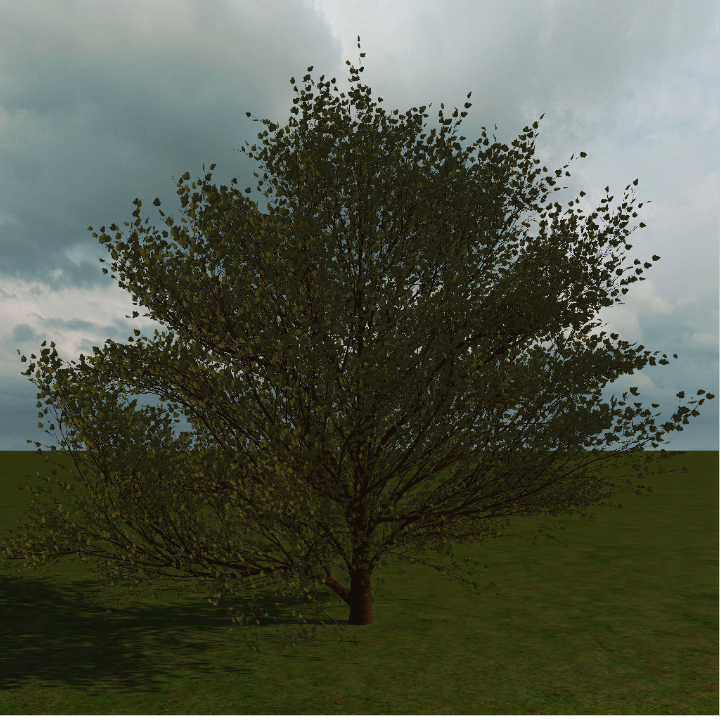
\includegraphics[height=6cm]{treegrowth3}

  			\caption{The development of a tree. a. 5 iterations, b. 15 iteration and c. 35 iterations. }
  			\label{fig:treegrowth}
  		\end{figure}
  	
  		Figure \ref{fig:pinebush} shows the versatility of the algorithm. It shows two trees that look quite different due to of the choice of parameters. The first tree looks more like a pine tree because of a higher \textit{alpha } value. The bushier tree to the right has a lower \textit{tropism} factor giving it the ability to reach higher and not be dragged down by gravity. A full list of differences between the two trees can be found in Table \ref{table:usedparam}. \\
  	
  		\begin{figure}[h!]
  			\centering
 			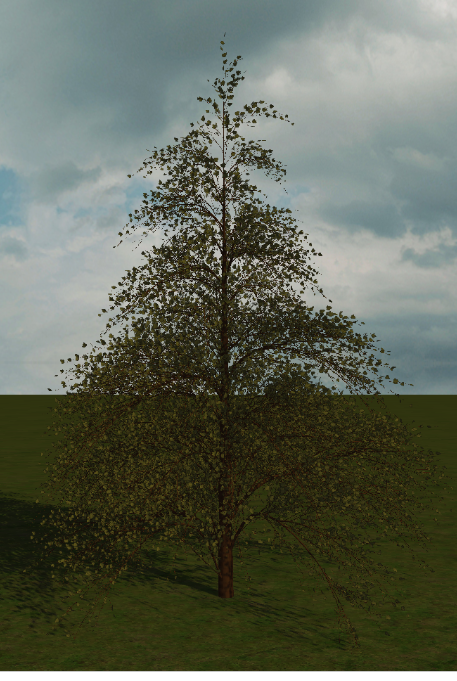
\includegraphics[height=6cm]{pine} 
 			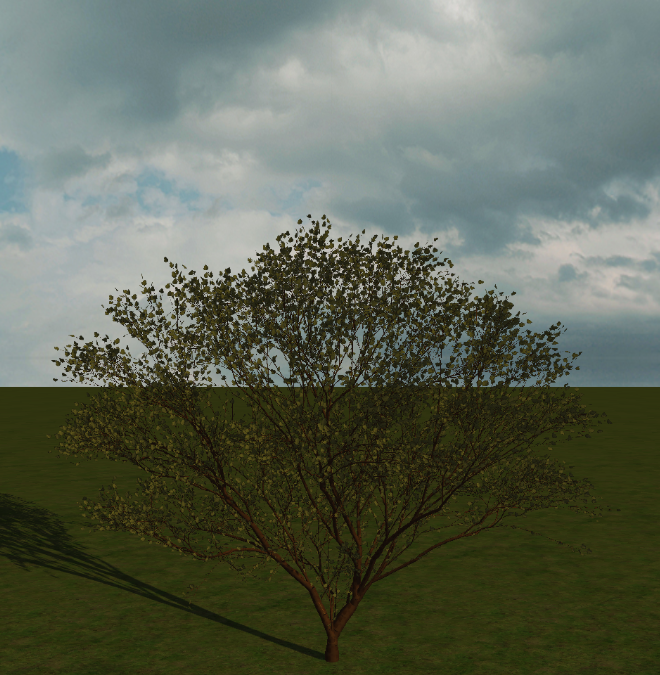
\includegraphics[height=6cm]{bush}
 			
  			\caption{Two trees with slightly different parameters. \textit{a.} A pine tree. b. A bush like tree.}
  			\label{fig:pinebush}
  		\end{figure}
  	
  		Figure \ref{fig:forest} shows a forest consisting of a number of trees. Each tree affect the growth of trees around them since they all share the same set of shadow voxels. Notice that the left tree in Figure \ref{fig:forest}a has been forces to grow to the left to find an area with more light. Both of the trees in Figure \ref{fig:forest}a has been grown the same number of iterations, but since the right tree was first, it received most of the available space. This shown the severe impact the shadow propagation system has on tree growth. \\
  	
	  	\begin{figure}[h!]
	  		\centering
	  		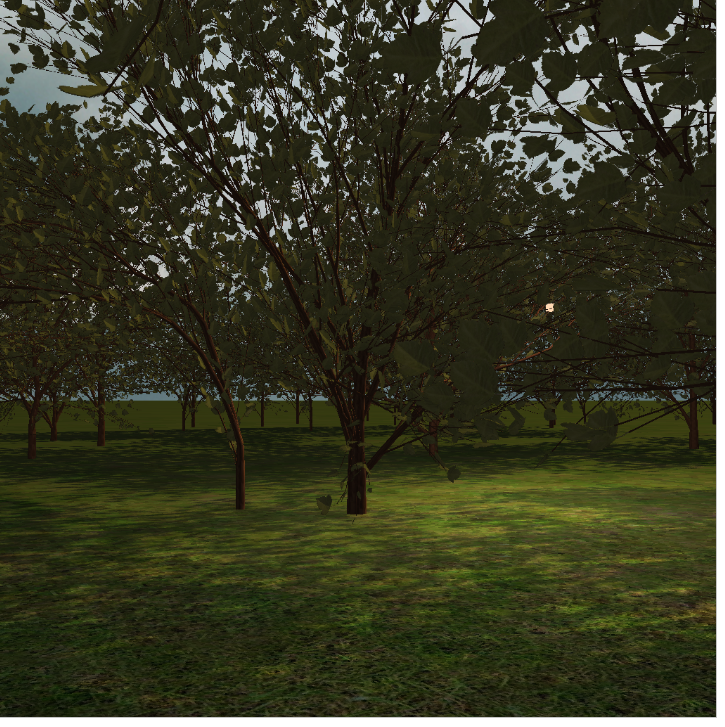
\includegraphics[height=6cm]{benttree}
	  		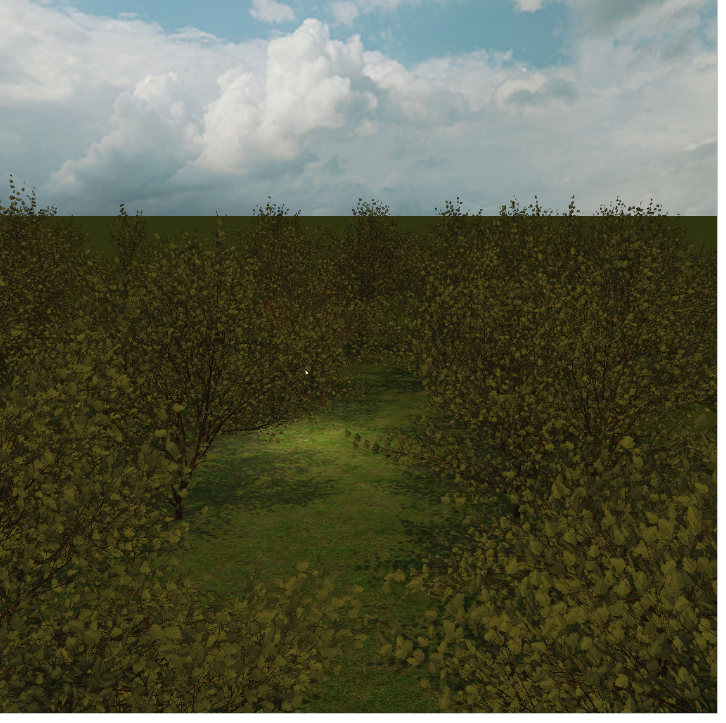
\includegraphics[height=6cm]{forrest}
	  		\caption{Example of a forest of many trees. 100 trees were placed randomly in the world.}
	  		\label{fig:forest}
	  	\end{figure}
	 
	 	The result of the volumetric light scattering postprocess can be seen in Figure \ref{fig:godrays}. The sun is mainly blocked by the branches passing through it. Leafs also block the light, but are made slightly transparent to generate a more realistic result. 
	 
		\begin{figure}[h!]
			\centering
		 	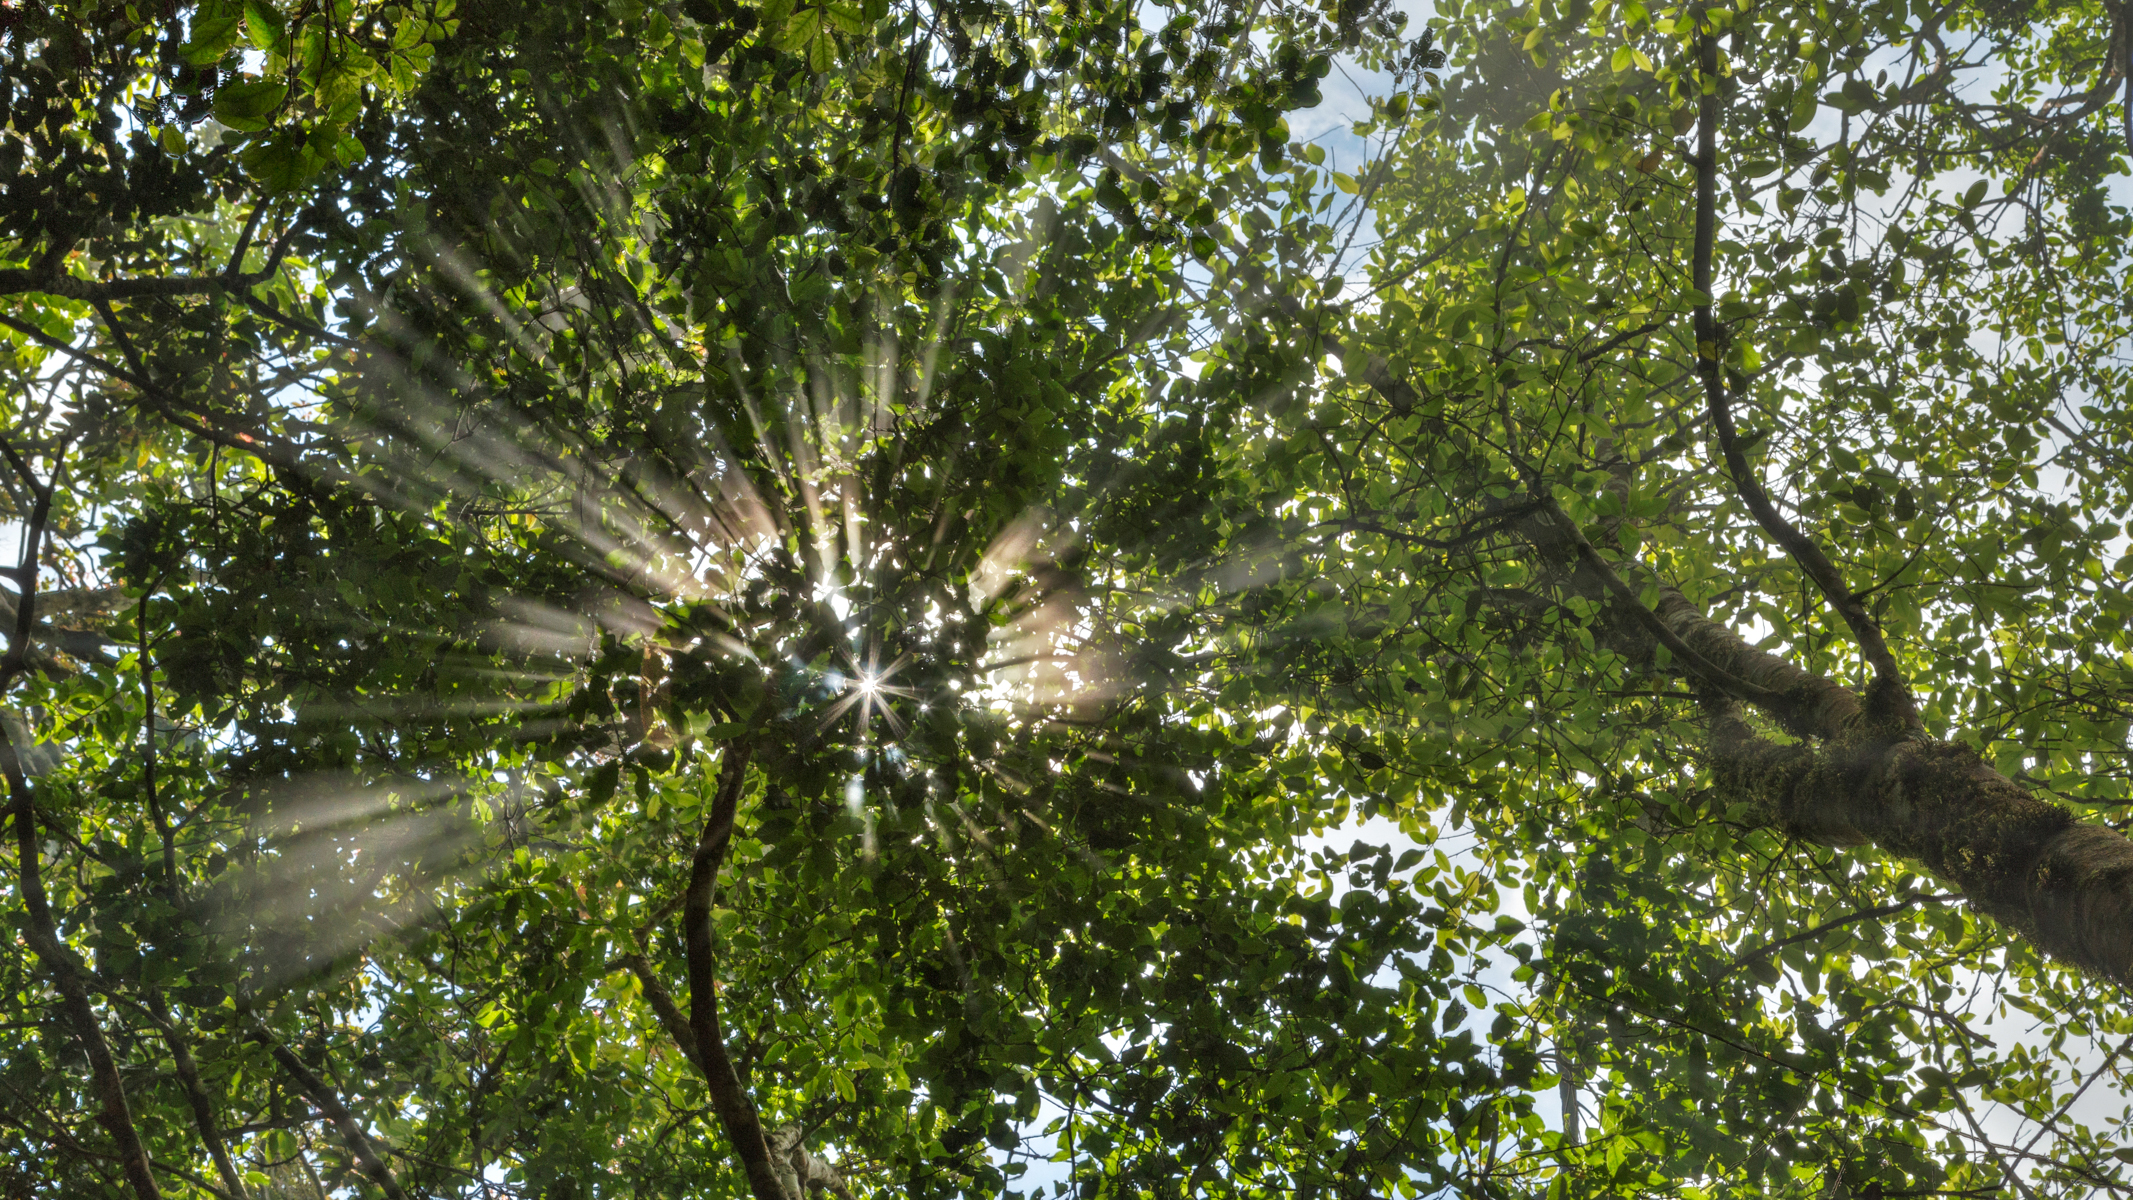
\includegraphics[height=10cm]{godrays}
		 	\caption{Sun shining through a tree resulting in volumetric light scattering. Parameters used in the postprocess: $exposure=0.05$, $decay=0.99$, $density=0.9$, $weight=1.5$, \textit{number of samples} $=170$.}
		 	\label{fig:godrays}
		\end{figure}
  	
  		\begin{table} [h!]
  			\begin{center}
  				\caption{Parameters used for trees in results.}
  				\begin{tabular}{  m{1cm} | P{0.5cm} P{0.5cm} P{0.5cm} P{0.5cm} P{0.5cm} P{0.5cm} P{0.5cm} P{0.5cm} P{0.5cm} } 
  					\hline
  					Tree & $\alpha$ & $\lambda$ & $\sigma$ & $\tau$ & BM & BE & $N_{min}$ & a & b \\
  					\hline
  					Fig \ref{fig:treegrowth} & 3 & 0.52 & 0.5 & 0.1 & 0.03 & 1.3 & 35 & 0.1 & 1.5 \\ 
  					Fig \ref{fig:pinebush}a & 2 & 0.5 & 0.1 & 0.3 & 0.03 & 1.3 & 35 & 0.1 & 1.7 \\ 
  					Fig \ref{fig:pinebush}b & 3 & 0.46 & 0.1 &  0.2 & 0.02 & 1.3 & 35 & 0.2 & 1.3\\ 
  					\hline
  				\end{tabular}
  				\label{table:usedparam}
  			\end{center}
  		\end{table}
  		
  	\section{Discussion}
  		
  		My method generates good looking given the right parameters. Finding good parameters is quite difficult and not suitable as the user interface for a finished product. This makes it hard to use the program in a more general way. The currently available parameters should be mapped to a set of more appropriate parameters for an end user. \\
  		
  		There are a number of problems with the tree generation that are worth discussing. The calculation of new branch directions is a combination of cure approximations of how real trees work. If realism is the goal, more research on the behavior of real trees is needed. Currently, a lot of branches has a nice curly look (see Figure \ref{fig:treegrowth}). While this looks pretty, I have yet to find a tree in nature that looks quite like that. \\
  		
  		The default length of a metamer is also a simplification that has been made. In this project, the metamer length is 50 cm, which is far larger that for most real trees. This simplification was made to decrease the number of nodes in a tree. Some tweaking is probably needed there. \\
  		
  		Speed is a relevant topic to discuss since the goal was to create real time growth of trees. Depending on the parameters, a tree with 25 iterations behind it can take up to 5 seconds to generate on a current mid range processor. Extrapolated to a whole scene, this might not be enough to realistically use the algorithm in a real time application. The speed could be increased by optimizing the algorithm and remove unnecessary recursions, or by doing parts of the recursion in parallel. \\
  		
  		On the topic of performance, the rendering speed should be addressed. On my system with only a few trees, the rendering is very smooth. More trees with more iterations could pose a problem for a real application. The optimizing  of leafs using instancing might not be enough to ensure a stable frame rate. Further optimizations could be implemented to increase performance. Level of details could be used and would likely have a large impact for large scenes. \\
  		
  		Figure \ref{fig:pinebush}a, while having the shape of a pine tree, does not look remotely like a pine tree. For this, more leaf assets and tree bark textures would be needed. This is something that would be quite easy to do (the infrastructure is in place to create trees with different assets) but I lacked the time (and skill) to create more models for leaves. \\
  		
  		Shadow mapping is a relatively cheap way to create good looking shadows. There are certainly more accurate methods, but you get what you pay for. Other methods such as shadow volumes or ray tracing give better results, but are a lot more demanding. Further discussions of shadow mapping has been done before, so I will leave that for more interesting problems. \\
  		
  		The post process volumetric light scattering gives impressive results for a relatively easy and fast implementation. Having sun bream constantly changing as the run pass through the treetops makes the scene come alive. Combined with the ever changing shadows, the scene feels real. There are still improvements that could be made. While the post process solution is cheap, it does not give perfect results. A more realistic volumetric approach could be implemented. We could calculate which part of the scene is lit by the sun and how much light should be reflected based on how much of the sun volume we pass through. This could quite easily be combined with the shadow volumes mentioned earlier. \\
  		
  		\subsection{Future Work}
  		
  			I see three areas for continued development for this project.\\
  			
  			Firstly, the algorithm needs to be optimized. As mentioned before, this could be done by calculating parts of the tree in parallel or by more traditional computer graphics solutions. \\
  			
  			Secondly, there are a number of topics concerning how real trees grow that are not addressed in the project. For example, the tropism factor is a crude simplification of the impact of gravity on three growth. A more robust system for handling the effect of external forces would be worth exploring.  \\
  			
  			Finally, it would be awesome of the current world is expanded with more visual improvements along the line of volumetric light scattering. I propose shadow volumes, lens flare and volumetric fog as areas to improve. There is a need for improved modeling of trees. As mentioned earlier, more leaf models and bark textures are needed. There is also room for improvement in the skinning of tree stems to handle more edge cases. \\
  	
  			I would also live to add that the rendering of leafs have a lot of room for improvement. In this project, leafs are rendered as solid object with a front side and a back side. This is not very realistic since the sun light shines through leafs most of the time. From what I can tell, there seams to be a lack of research into this topic.

	\newpage
	\bibliographystyle{plainnat}
	\bibliography{ref}{}
	
	\newpage
	\appendix
	\section{Shader code for volumetric light scattering}
	\label{appendix:godray}
		
	\begin{lstlisting}[basicstyle=\ttfamily\footnotesize, tabsize=4]
	vec2 delta_tex_coord = vec2(out_tex_coords - sun_pos);
	delta_tex_coord *= 1.0 / float(NUM_SAMPLES) * density;
	
	vec2 tex_coord = out_tex_coords;
	
	float illumination_decay = 1.0;
	vec4 godray_color = vec4(0,0,0,0);
	
	for(int i = 0; i < NUM_SAMPLES; i++)
	{
		tex_coord -= delta_tex_coord;
		
		vec4 s = texture(god_ray_pass, tex_coord);
		
		s *= illumination_decay * weight;
		
		godray_color += s;
		
		// Update exponential decay factor.
		illumination_decay *= decay;
	}
	
	return godray_color * exposure;
	\end{lstlisting}
		
	\section{Shader code for shadow map calculation}
	\label{appendix:shadow}
		
	\begin{lstlisting}[basicstyle=\ttfamily\footnotesize, tabsize=4]
	vec3 proj_coords = frag_pos_light_space.xyz / frag_pos_light_space.w;
	proj_coords = proj_coords * 0.5 + 0.5;

	float current_depth = proj_coords.z;
	
	float bias = max(0.005 * (1.0 - dot(normal, light_dir)), 0.00005);
	float shadow = 0.0;
	vec2 texel_size = 1.0 / textureSize(shadow_map, 0);
	for(int x = -1; x <= 1; ++x)
	{
		for(int y = -1; y <= 1; ++y)
		{
			float depth = texture(shadow_map, proj_coords.xy + vec2(x, y) * texel_size).r; 
			shadow += current_depth - bias > depth ? 1.0 : 0.0;        
		}
	}
	shadow /= 9.0;
	
	if(proj_coords.z > 1.0)
		shadow = 0.0;
	
	return shadow;
		
	\end{lstlisting}
  	
\end{document}
